\chapter{Estado del Arte}


\section{Librerías de visualización de estructuras de datos}

Actualmente existen varias librerías para generar visualizaciones de estructuras de datos, pero muchas de ellas están implementadas en lenguajes distintos de Python y no están diseñadas para poder ser utilizadas en Notebooks.
Un ejemplo de esto es la librería Reftree~\cite{Stanch2021} que permite crear visualizaciones de estructuras de datos, pero en el lenguaje Scala, por lo tanto, no se puede utilizar para visualizar estructuras de datos implementadas en Python y tampoco se puede utilizar en Jupyter Notebooks.
Otro ejemplo es la librería Lolviz~\cite{Lolviz} que, si bien si permite visualizar en Notebooks estructuras de datos implementadas en Python, cuenta con la limitación de que no puede generar animaciones. En la figura \ref{fig:comparacion} se pueden ver ejemplos de las visualizaciones generadas por estas librerías.

\begin{figure}[h]%
    \centering
    \subfloat[Reftree]{
        \centering
        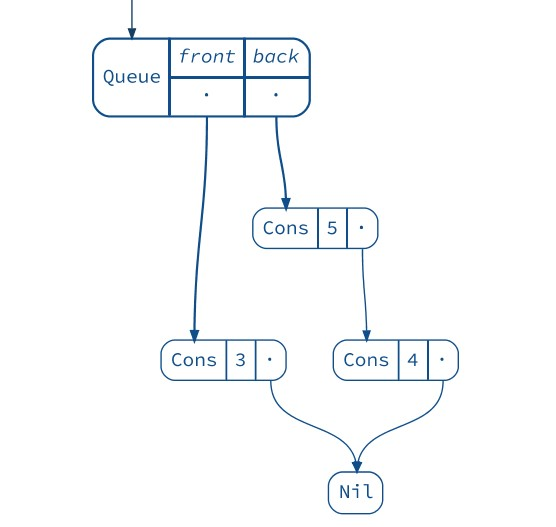
\includegraphics[width=\dimexpr(\linewidth-40pt)/2\relax, height=\dimexpr(\linewidth-40pt)/2\relax]{imagenes/ejemplos/reftree}
        \label{fig:reftree}
    }\qquad
    \subfloat[Lolviz]{
        \centering
        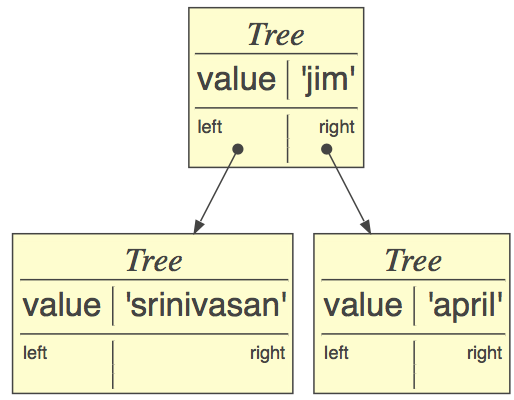
\includegraphics[width=\dimexpr(\linewidth-40pt)/2\relax]{imagenes/ejemplos/lolviz}
        % \vspace{38px}
        \label{fig:lolviz}
    }\\
    \subfloat[Aed Utilities]{
        \centering
        \includesvg[width=\dimexpr(\linewidth-40pt)/2\relax]{imagenes/ejemplos/aed}
        \label{fig:aed}
    }\qquad
    \subfloat[Manim]{
        \centering
        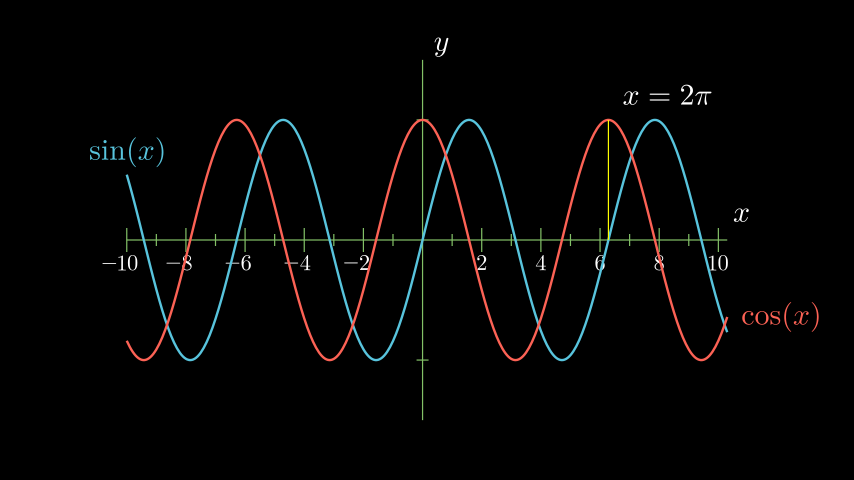
\includegraphics[width=\dimexpr(\linewidth-40pt)/2\relax]{imagenes/ejemplos/manim}
        \label{fig:manim}
    }
    \caption{Ejemplos de visualizaciones generadas por las distintas herramientas. Obtenidas de \cite{Stanch2021}, \cite{Lolviz}, \cite{aed-utilities} y \cite{manim}, respectivamente.}
    \label{fig:comparacion}
\end{figure}

Por otro lado, existe la librería Aed-Utilities~\cite{aed-utilities} creada para el curso de Algoritmos y Estructuras de Datos de la FCFM por el Profesor Ivan Sipiran; que, si bien permite generar diagramas de estructuras de datos en Python y mostrarlas en un Notebook, cuenta con las siguientes limitaciones: no permite crear animaciones, la API no es muy cómoda de utilizar y el algoritmo que utiliza para generar las visualizaciones es poco eficiente. % TODO: Explicar

Tanto Aed-Utilites como Lolviz generan los diagramas utilizando Graphviz ---una herramienta originalmente desarrollada por AT\&T para dibujar gráficos especificados en el lenguaje DOT--- que permite generar diagramas de muy buena calidad, pero no permite crear animaciones.

En cuanto a las herramientas para generar animaciones, existe la librería Manim~\cite{manim}, diseñada para generar visualizaciones animadas de matemáticas. Si bien no está diseñada para crear visualizaciones de estructuras de datos, es relevante porque permite generar animaciones y estas animaciones se pueden ver desde Notebooks. Esta librería tiene un diseño orientado a objetos, donde una animación es un objeto que tiene un campo con el objeto matemático que representa y tiene un método que permite animar el objeto según una función de interpolación. Para generar el resultado final puede utilizar varios back-ends de rendering, incluyendo OpenGL y WebGL. Utilizando este último cuando se usa desde un Notebook. En la figura \ref{fig:manim} se puede ver una visualización de una función creada con esta herramienta.

Otra herramienta enfocada en las matemáticas es Penrose~\cite{Penrose}, una herramienta que permite crear diagramas a partir de un programa en un lenguaje específico de dominio. La disposición de los elementos en el diagrama se obtiene mediante optimización numérica. El lenguaje específico de dominio (o DSL por sus iniciales en inglés) se separa en un archivo que define solo la parte matemática y en otro que define el estilo.

Dado que no se encontró ninguna herramienta existente que permita visualizar estructuras de datos implementadas en Python, permita generar animaciones y permita mostrar las visualizaciones generadas en un Jupyter Notebooks, se requiere crear una nueva librería que implemente esta funcionalidad.

\section{Jupyter Notebooks}

Los Jupyter Notebooks son archivos interactivos que almacenan bloques de texto, código y también pueden contener imágenes, videos y animaciones interactivas. Un Jupyter Notebook tiene varios componentes que permiten construir la experiencia de usuario. En primer lugar, está el archivo del notebook que es un archivo JSON con la extensión \texttt{.ipynb}, que almacena en el disco todos los datos persistentes del notebook, incluyendo los bloques de texto, los bloques de código y sus salidas, las imágenes, etc. Después, está el \textit{kernel} o núcleo, que es un intérprete del lenguaje respectivo, con la capacidad de comunicarse con el servidor del notebook. El servidor del notebook se encarga de la comunicación entre el front-end, el kernel y el archivo del notebook. Finalmente, está el front-end del notebook, que se encarga de mostrarle al usuario una representación del notebook y le permite a este interactuar con el notebook, usualmente corresponde a un navegador web. En la figura \ref{fig:notebook_arq} se puede ver un diagrama de esta arquitectura.

\begin{figure}[h]
  \centering
  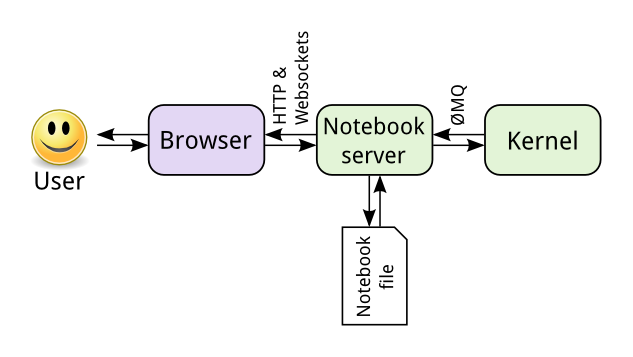
\includegraphics[width=0.8\linewidth]{imagenes/notebook/notebook_components}
  \caption{Arquitectura de Jupyter Notebooks. Obtenido de \cite{arq-notebook}.}
  \label{fig:notebook_arq}
  \centering
\end{figure}

Existen múltiples kernels, uno por cada lenguaje que soportan los Jupyter Notebooks, pero el más conocido es el kernel IPython que es el kernel del lenguaje Python. IPython además de ser un kernel de Jupyter Notebooks es un intérprete interactivo de Python, con funcionalidades como contenido multimedia y completado de comandos. Cuando se utiliza un notebook con el lenguaje Python, el servidor del notebook se comunica con este intérprete que es que se encarga de interpretar los bloques de código y responder con la salida generada cuando el servidor del notebook envía el request.

Para crear componentes interactivos en un Notebook de Python se utiliza la librería Jupyter Widgets. Esta librería permite definir un modelo que representa el componente, y una vista en JavaScript y HTML que es mostrada por el front-end del Notebook. El modelo se define tanto en JavaScript como en Python y la librería se encarga de mantener las dos versiones sincronizadas. Para mantener las dos versiones sincronizadas, es necesario serializar y deserializar los campos del modelo, para poder enviarlos en formato JSON. Entonces, para los campos sencillos, la librería se puede encargar de la serialización o deserialización, pero para los casos más complejos se deben definir manualmente los serializadores y deserializadores para cada campo. En la figura \ref{fig:widget_arq} se observa la arquitectura de un widget generado con esta librería.

\begin{figure}[h]
  \centering
  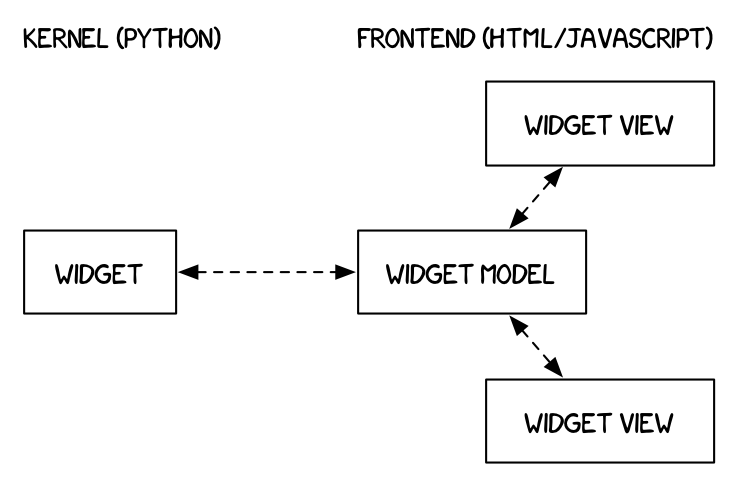
\includegraphics[width=0.8\textwidth]{imagenes/notebook/WidgetModelView}
  \caption{Arquitectura de Jupyter Widgets. Obtenido de \cite{arq-widget}.}
  \label{fig:widget_arq}
  \centering
\end{figure}

\section{ThreeJS}

ThreeJS es una librería de JavaScript de gráficos en 3D que utiliza WebGL. WebGL es una API de JavaScript parte de los estándares web que permite el uso de la GPU para el rendering y el uso de shaders escritos en GLSL ES (OpenGL ES  Shading Language). La API de ThreeJS es de más alto nivel que WebGL, facilitando la programación de gráficos. Adicionalmente a lo que tiene WebGL implementa escenas, luces, materiales, sombras, entre otros~\cite{threejs-manual}.

Para renderizar gráficos en ThreeJS se deben definir lo siguientes elementos: escena, cámaras, geometrías, materiales, objetos, controles y renderers. Teniendo esto se deben agregar los objetos a ser mostrados al grafo de escena y la función de rendering debe ser agregada a un loop, para que se actualice la escena si hay cambios en las propiedades de los objetos. En la figura \ref{fig:threejs-structure} se puede ver un diagrama que muestra los elementos que componen una escena en ThreeJS.

\begin{figure}[h]
  \centering
  \includesvg[width=0.8\textwidth]{imagenes/threejs/threejs-structure}
  \caption{Estructura de una escena en ThreeJS. Obtenido de \cite{threejs-manual}.}
  \label{fig:threejs-structure}
  \centering
\end{figure}

Además, ThreeJS cuenta con un sistema de animaciones donde se pueden crear animaciones para objetos en el grafo de escena. Para esto primero se debe definir una AnimationAction que está compuesta por un KeyframeTrack y una cadena de texto con el nombre o UUID del objeto en el grafo de escena a ser animado y la propiedad de este a ser animada con el KeyframeTrack. El KeyframeTrack se genera a partir de un arreglo de los valores con la propiedad a ser modificada y un arreglo con los tiempos correspondientes a esos valores. Además, existen los AnimationMixers que permiten mezclar distintas animation actions sobre un mismo objeto en el grafo de escena. Lo que finalmente se usa para crear la animación es un AnimationClip, que se obtiene aplicando una AnimationAction a un AnimationMixer.

Una ventaja de esta librería es que como usa WebGL que es un estándar web, los gráficos generados con esta librería pueden ser vistos por todos los usuarios con navegadores compatibles. Además, según caniuse.com el 99.97\% de los usuarios utiliza navegadores compatibles con WebGL.
